\begin{frame}
  \frametitle{Physical Structure}

  The geometry of Microwave Bipolar Transistors are important because they operate in high frequencies. The \emph{inter digitated geometry} consists of a large number of emitter strips alternating with base strips. The \emph{overlay geometry} has a large number of segmented emitters overlaid through a number of wide metal strips. The \emph{matrix/ mesh geometry}has an emitter that forms the grid, the base filling the meshes of this grid with a $p^+$ contact area in the middle of each mesh.
  Inter-digitated structure is suitable for small signal applications in the L, S and C bands whereas overlay and matrix structures are useful as power devices in VHF and UHF regions.
\end{frame}

\begin{frame}
  \begin{figure}[h]
    \caption{Geometrical Structures of microwave power transitor}
    \centering
    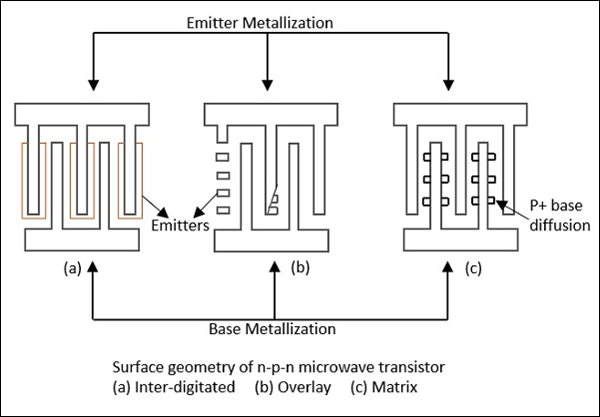
\includegraphics[width=0.4\textwidth]{./images/chapter9/fig9_1.png}
  \end{figure}
\end{frame}